\documentclass{article}
\usepackage{graphicx}
\usepackage{xcolor}
\usepackage{array}
\usepackage[T1]{fontenc}
\usepackage{bbding}
\usepackage{amsfonts}
\usepackage{amsmath}
\usepackage{pgfgantt}
\usepackage[margin=2cm]{geometry}
\usepackage[hidelinks]{hyperref}
\usepackage{subcaption}
\usepackage{float}
\newcommand\Tstrut{\rule{0pt}{2.6ex}}
\newcommand\Bstrut{\rule[-0.9ex]{0pt}{0pt}}
\newcommand{\TBstrut}{\Tstrut\Bstrut}
\renewcommand{\contentsname}{Sommaire}
\newcommand{\stepimage}[3][0.3\textwidth]{%
  \minipage{#1}
    \includegraphics[width=\linewidth]{ressources/#2}
    \caption{#3}
  \endminipage\hfill
}

\title{OCR}
\author{}
\date{}

\begin{document}

\maketitle
\tableofcontents

\newpage



\section{Extraction de la grille et des mots}

Nous prendrons comme exemples 3 images, de chaque niveau.

\begin{figure}[!htb]
    \minipage{0.30\textwidth}
      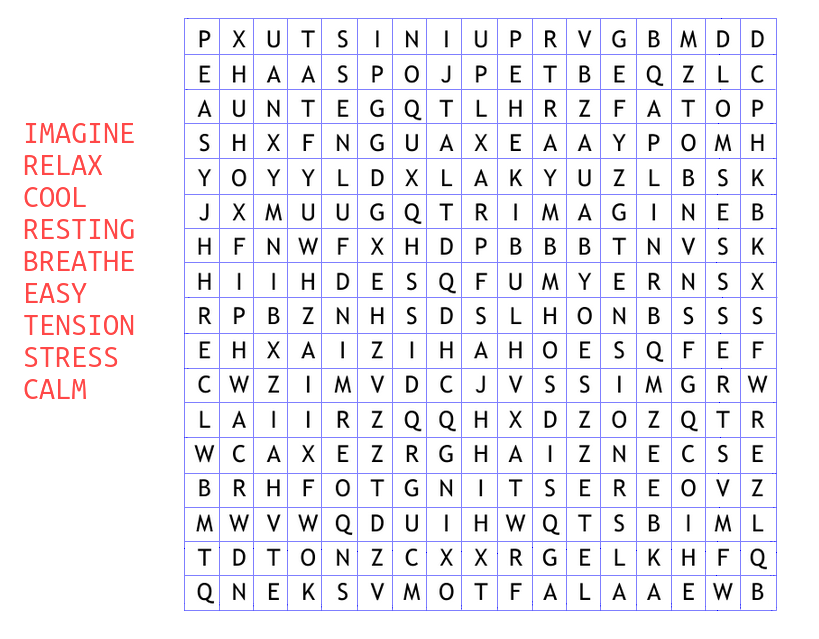
\includegraphics[width=\linewidth]{images/level_1_image_1.png}
      \caption{}
    \endminipage\hfill
    \minipage{0.33\textwidth}
      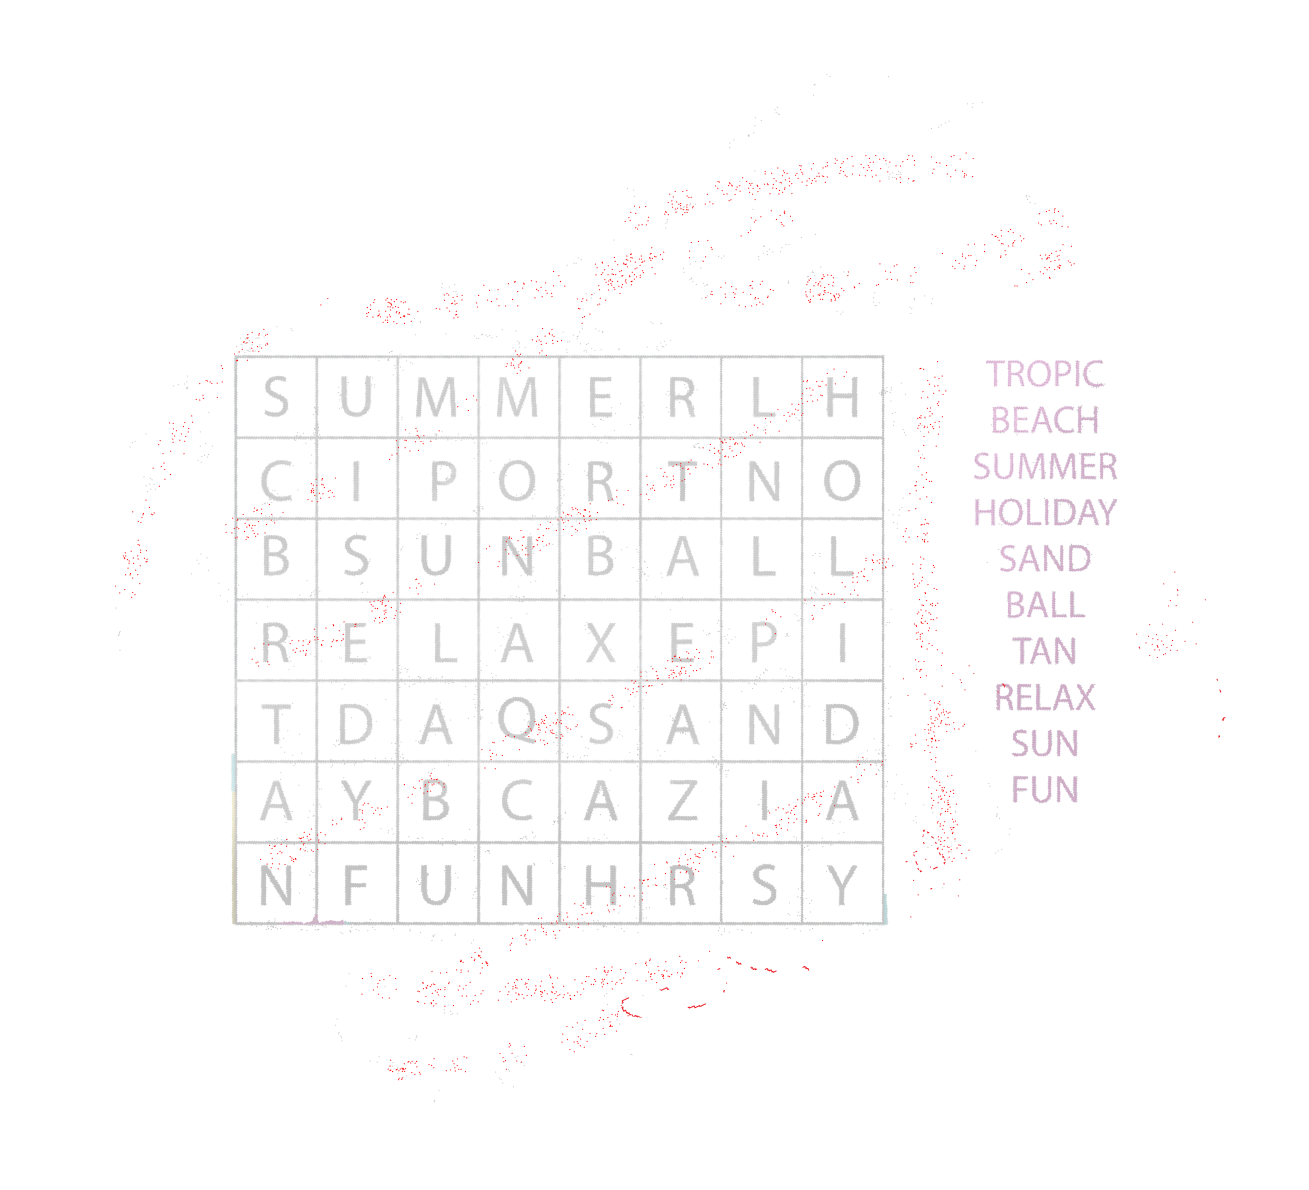
\includegraphics[width=\linewidth]{images/level_2_image_1_rotated_25.0deg.png}
      \caption{}
    \endminipage\hfill
    \minipage{0.26\textwidth}%
      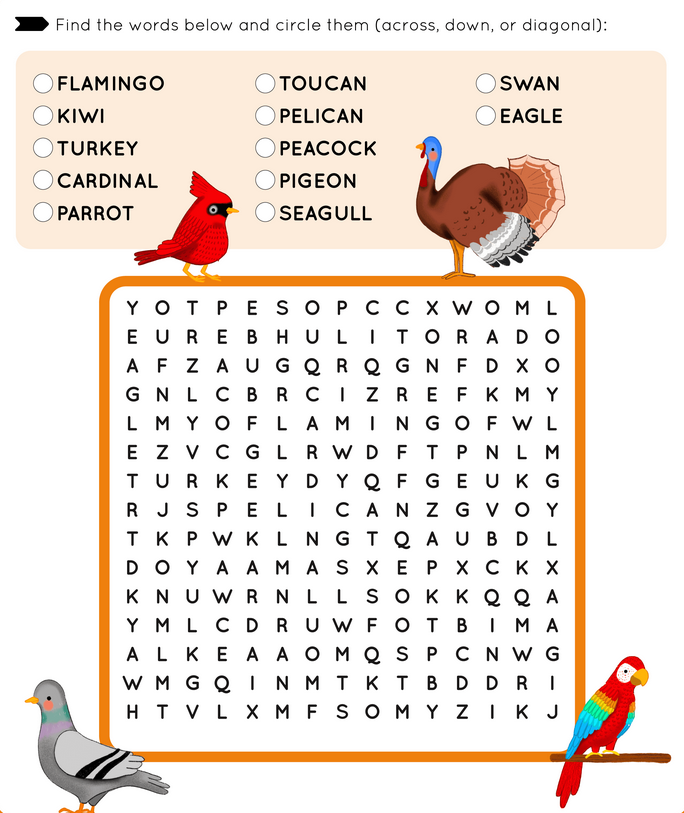
\includegraphics[width=\linewidth]{images/level_3_image_2.png}
      \caption{}
    \endminipage
\end{figure}


\subsection{Chargement des images}

Le chargement des images est réalisé à l'aide de GTK, qui gère le chargement et la manipulation des fichiers image.

\subsection{Extraction de la grille}

Après avoir chargé l'image, on commence par la pré-traitement de l'image pour la rendre plus facile à traiter.

\subsubsection{Transformation en niveaux de gris}
\begin{figure}[!htb]
    \stepimage[0.30\textwidth]{1step_01_grayscale.png}{}
    \stepimage[0.33\textwidth]{2step_01_grayscale.png}{}
    \stepimage[0.26\textwidth]{3step_01_grayscale.png}{}
\end{figure}
On commence par transformer l'image en niveaux de gris pour la rendre plus facile à traiter.
En utilisant la formule de luminance standard :

\[
Y = 0.299 \cdot R + 0.587 \cdot G + 0.114 \cdot B
\]

Où $R$, $G$ et $B$ sont les valeurs des composantes rouge, vert et bleu de l'image.


\subsection{Débruitage adaptatif}
\begin{figure}[!htb]
    \stepimage[0.30\textwidth]{1step_02_adaptive_denoise.png}{}
    \stepimage[0.33\textwidth]{2step_02_adaptive_denoise.png}{}
    \stepimage[0.26\textwidth]{3step_02_adaptive_denoise.png}{}
\end{figure}
Pour adapter le débruitage à chaque image, nous devons d'abord estimer son niveau de bruit. Cette estimation est réalisée en analysant la variance locale de l'intensité des pixels. La méthode se décompose en plusieurs étapes :

\paragraph{1. Échantillonnage de fenêtres locales}
On sélectionne un ensemble de petites fenêtres \(W_s\) (de \(N\) pixels chacune) à travers l'image, centrées en des points (s). Par exemple, une fenêtre de \(3 \times 3\) pixels contient \(N=9\) pixels.

\paragraph{2. Calcul de la moyenne et de la variance locales}
Pour chaque fenêtre \(W_s\), on calcule d'abord l'intensité moyenne des pixels \(\mu_s\) :
\[
\mu_s = \frac{1}{N} \sum_{p \in W_s} I(p)
\]
Ensuite, on calcule la variance locale \(v_s\), qui mesure la dispersion des intensités autour de la moyenne :
\[
v_s = \frac{1}{N} \sum_{p \in W_s} \big(I(p) - \mu_s\big)^2
\]

\paragraph{3. Estimation de la variance du bruit}
La variance du bruit dans l'image, notée \(\sigma_{\text{bruit}}^{2}\), est estimée en faisant la moyenne de toutes les variances locales calculées à l'étape précédente :
\[
\sigma_{\text{bruit}}^{2} = \frac{1}{|S|} \sum_{s \in S} v_s
\]

\paragraph{4. Normalisation du niveau de bruit}
Enfin, pour obtenir un paramètre utilisable par l'algorithme de débruitage, on normalise cette variance pour obtenir un niveau de bruit \(\eta\) compris entre 0 et 1 :
\[
\eta = \min\!\left(1, \; \frac{\sigma_{\text{bruit}}^{2}}{1000}\right)
\]

\paragraph{Application du filtre gaussien}
En fonction du niveau de bruit \(\eta\) calculé, un filtre de flou gaussien avec des paramètres variables est appliqué :
\begin{itemize}
    \item Si $\eta < 0.1$ (bruit faible) : un noyau de \(3 \times 3\) avec \(\sigma = 0.5\) est utilisé.
    \item Si $0.1 \leq \eta < 0.3$ (bruit modéré) : un noyau de \(3 \times 3\) avec \(\sigma = 1.0\) est utilisé.
    \item Si $\eta \geq 0.3$ (bruit élevé) : un noyau de \(5 \times 5\) avec \(\sigma = 1.5\) est utilisé.
\end{itemize}
L'opération de flou gaussien est définie par :
\[
\operatorname{GaussianBlur(Image, k, \sigma)}[x,y] = \sum_{i=-r}^{r} \sum_{j=-r}^{r} w_{i,j}\, Image[x-i, y-j]
\]
où \(k\) est la taille du noyau (\(r = (k-1)/2\)), \(\sigma\) est l'écart-type, et \(w_{i,j}\) sont les poids du noyau gaussien :
\[
w_{i,j} = \frac{\exp\!\left(-\dfrac{i^{2}+j^{2}}{2\,\sigma^{2}}\right)}{\displaystyle \sum_{u=-r}^{r} \sum_{v=-r}^{r} \exp\!\left(-\dfrac{u^{2}+v^{2}}{2\,\sigma^{2}}\right)}
\]

\subsection{Seuil adaptatif}
\begin{figure}[!htb]
    \stepimage[0.30\textwidth]{1step_03_threshold.png}{}
    \stepimage[0.33\textwidth]{2step_03_threshold.png}{}
    \stepimage[0.26\textwidth]{3step_03_threshold.png}{}
\end{figure}
Le seuillage est une technique fondamentale pour binariser une image, c'est-à-dire la convertir en une image en noir et blanc. Un seuillage global simple, qui utilise une seule valeur de seuil pour tous les pixels, est souvent inefficace sur des images avec des variations d'éclairage ou du bruit. Le seuillage adaptatif résout ce problème en calculant un seuil différent pour chaque pixel, en se basant sur une petite région environnante.

Pour un pixel donné à la position \((x, y)\) dans l'image \(I\), le seuil \(T(x, y)\) est calculé en analysant l'intensité des pixels dans un voisinage de taille \texttt{block\_size} \(\times\) \texttt{block\_size}, centré sur \((x, y)\). On utilisera deux méthodes pour calculer ce seuil local.

\subsubsection{Méthode de la moyenne}
Dans cette méthode, le seuil \(T(x, y)\) est simplement la moyenne des intensités des pixels dans le voisinage, à laquelle on soustrait une constante \(C\).

\[
T(x, y) = \frac{1}{N} \sum_{(i, j) \in W_{xy}} I(i, j) - C
\]

Où :
\begin{itemize}
    \item \(W_{xy}\) est la fenêtre de voisinage de taille \texttt{block\_size} \(\times\) \texttt{block\_size} centrée en \((x, y)\).
    \item \(N\) est le nombre total de pixels dans cette fenêtre (\(N = \texttt{block\_size}^2\)).
    \item \(I(i, j)\) est l'intensité du pixel à la position \((i, j)\).
\end{itemize}

\subsubsection{Méthode Gaussienne}
Cette méthode est une version plus sophistiquée où le seuil est une somme pondérée des intensités des pixels du voisinage. Les pixels plus proches du centre de la fenêtre ont plus d'influence sur le calcul du seuil. Les poids sont déterminés par un noyau gaussien.

\[
T(x, y) = \sum_{(i, j) \in W_{xy}} w(i, j) \cdot I(i, j) - C
\]

Où les poids \(w(i, j)\) sont dérivés d'un noyau gaussien et normalisés pour que leur somme soit égale à 1.

\subsubsection{Application du seuil}
Une fois le seuil \(T(x, y)\) calculé pour chaque pixel, l'image de sortie \(I_{\text{out}}\) est générée en appliquant l'une des deux règles suivantes :
\begin{itemize}
    \item \textbf{\texttt{THRESH\_BINARY}}:
    \[
    I_{\text{out}}(x, y) =
    \begin{cases}
    \text{max\_value} & \text{si } I(x, y) > T(x, y) \\
    0 & \text{sinon}
    \end{cases}
    \]
    \item \textbf{\texttt{THRESH\_BINARY\_INV}}:
    \[
    I_{\text{out}}(x, y) =
    \begin{cases}
    0 & \text{si } I(x, y) > T(x, y) \\
    \text{max\_value} & \text{sinon}
    \end{cases}
    \]
\end{itemize}


\subsection{Detection de la grille}
\begin{figure}[!htb]
    \stepimage[0.30\textwidth]{1step_05_grid_extraction.png}{}
    \stepimage[0.33\textwidth]{2step_05_grid_extraction.png}{}
    \stepimage[0.26\textwidth]{3step_05_grid_extraction.png}{}
\end{figure}

Une fois l'image binarisée, l'étape suivante consiste à localiser et à extraire la grille. Notre approche repose sur l'analyse des formes géométriques présentes dans l'image, en partant de l'hypothèse que la grille est l'objet le plus grand et le plus remarquable.

\subsubsection{1. Recherche des contours}
La première étape est d'identifier les contours de tous les objets dans l'image binarisée. Un contour est une séquence de pixels qui trace la frontière d'une forme. Pour ce faire, un algorithme de suivi de bordure (inspiré de l'algorithme de Suzuki) est utilisé. Son fonctionnement peut se résumer en plusieurs étapes clés :

\begin{enumerate}
    \item \textbf{Balayage de l'image :} L'algorithme parcourt l'image de gauche à droite et de haut en bas, à la recherche d'un pixel appartenant à un objet (un pixel blanc) qui n'a pas encore été assigné à un contour.

    \item \textbf{Initialisation du suivi :} Lorsqu'un tel pixel est trouvé, il est marqué comme le point de départ d'un nouveau contour. L'algorithme commence alors à examiner ses 8 pixels voisins (voisinage de Moore) dans un ordre prédéfini (par exemple, dans le sens horaire) pour trouver le prochain pixel appartenant à la bordure.

    \item \textbf{Suivi de la bordure :} Une fois le pixel suivant trouvé, l'algorithme s'y "déplace" et l'ajoute à la liste des points du contour. Depuis ce nouveau point, il répète le processus de recherche dans le voisinage pour trouver le pixel suivant, en s'assurant de suivre la frontière de l'objet. Ce processus est analogue à celui d'une personne qui suivrait un mur en gardant une main dessus.

    \item \textbf{Condition d'arrêt :} Le suivi se poursuit jusqu'à ce que l'algorithme revienne à son point de départ initial. À ce moment, le contour est considéré comme complet et est ajouté à la liste des contours trouvés.

    \item \textbf{Itération :} L'algorithme reprend ensuite son balayage initial de l'image pour trouver le point de départ d'un autre objet non encore traité. Le processus se répète jusqu'à ce que tous les pixels de l'image aient été visités.
\end{enumerate}

Le résultat final est une liste exhaustive de tous les contours présents dans l'image, chacun étant représenté par une liste de points qui définissent sa forme.

\subsubsection{2. Identification du plus grand contour}
Après avoir obtenu la liste de tous les contours, nous devons identifier celui qui correspond à la grille. L'heuristique utilisée est simple : la grille est supposée être le plus grand objet connexe de l'image. Par conséquent, nous calculons l'aire de chaque contour détecté et nous sélectionnons celui qui a la plus grande superficie.

\subsubsection{3. Calcul de la boîte englobante (Bounding Box)}
Le contour identifié peut avoir une forme légèrement irrégulière. Pour faciliter l'extraction, nous calculons le plus petit rectangle droit (non incliné) qui englobe complètement ce contour. Ce rectangle, appelé "boîte englobante", nous fournit les coordonnées \((x, y)\) du coin supérieur gauche ainsi que la largeur et la hauteur de la grille.

\subsubsection{4. Extraction de la grille}
Avec les coordonnées de la boîte englobante, nous pouvons maintenant "rogner" ou extraire la région de la grille de l'image d'origine (celle en niveaux de gris, avant le seuillage). Cela nous donne une nouvelle image ne contenant que la grille, prête pour une analyse plus approfondie.\\\\
Cependant nous remarquons, notamment sur la dernière image, que la grille n'est pas parfaitement extraite. Nous appliquerons par la suite un deuxième algorithme de detection de la grille, qui nous permettra d'extraire la grille de manière plus précise.

\subsection{Nettoyage morphologique de la grille}

\begin{figure}[!htb]
  \stepimage[0.30\textwidth]{1step_07_cleaned_grid.png}{}
  \stepimage[0.33\textwidth]{2step_07_cleaned_grid.png}{}
  \stepimage[0.26\textwidth]{3step_07_cleaned_grid.png}{}
\end{figure}
L'image de la grille extraite à l'étape précédente n'est pas toujours parfaite. Elle peut contenir de petits trous ou des coupures dans les lignes, principalement à cause du bruit ou des lettres qui touchent les bords de la grille. Pour améliorer la qualité de la grille en vue de l'analyse des cellules, nous appliquons une opération de nettoyage appelée \texttt{fermeture morphologique} (\textit{Morphological Closing}).

Cette opération combine deux étapes fondamentales :
\begin{enumerate}
    \item \textbf{La dilatation :}
    Cette opération a pour effet d'épaissir ou d'agrandir les régions blanches de l'image. Son principal intérêt est de combler les petits trous à l'intérieur des objets et de reconnecter des parties d'un même objet qui auraient été séparées par du bruit.

    \paragraph{Au niveau du pixel :} L'opération fonctionne avec un "élément structurant", qui est une petite matrice (un noyau, ici de 2x2) que l'on fait glisser sur toute l'image. Pour chaque pixel de l'image de sortie, on effectue le test suivant :
    \begin{itemize}
        \item On centre l'élément structurant sur la position correspondante dans l'image d'origine.
        \item Si \textbf{au moins un} des pixels de l'image d'origine couverts par l'élément structurant est blanc, alors le pixel de l'image de sortie devient blanc.
    \end{itemize}
    Le résultat est que les frontières des objets blancs s'étendent, les petits trous noirs se comblent, et les éléments proches peuvent fusionner.

    \item \textbf{L'érosion :}
    C'est l'opération inverse de la dilatation. Elle a pour effet d'amincir ou de rétrécir les régions blanches. Elle est principalement utilisée pour éliminer les petites taches de bruit blanc et pour séparer des objets qui ne sont que faiblement connectés.

    \paragraph{Au niveau du pixel :} L'érosion utilise le même élément structurant, mais la règle est plus stricte :
    \begin{itemize}
        \item On centre l'élément structurant sur la position correspondante dans l'image d'origine.
        \item Le pixel de l'image de sortie devient blanc \textbf{uniquement si tous} les pixels de l'image d'origine couverts par l'élément structurant sont blancs. Si un seul de ces pixels est noir, le pixel de sortie devient noir.
    \end{itemize}
    Le résultat est que les objets blancs rétrécissent, les fines connexions sont coupées et les petites taches de bruit blanc sont éliminées. Appliquée après la dilatation, elle permet de retrouver la taille initiale des lignes de la grille tout en gardant les bénéfices du nettoyage.
\end{enumerate}

L'effet net de la fermeture est de nettoyer la grille en supprimant le bruit "noir" (les petits trous) à l'intérieur des lignes blanches, sans altérer de manière significative la structure générale de la grille.

\subsection{Analyse de la Structure de la Grille}

Après avoir isolé et nettoyé l'image de la grille, l'objectif est de la segmenter en cellules individuelles, chacune contenant une seule lettre. L'approche pour y parvenir dépend de la nature de la grille elle-même : certaines grilles sont dessinées avec des lignes internes séparant chaque cellule, tandis que d'autres ne contiennent que les lettres. Notre algorithme doit donc gérer ces deux cas distincts.
Cette analyse de la structure interne vient ainsi affiner et compléter l'extraction globale de la grille vue précédemment, en nous permettant d'identifier précisément chaque cellule.

\subsubsection{Cas 1 : Grille avec lignes internes (Détection par Lignes)}

\begin{figure}[H]
  \centering
  \minipage{0.30\textwidth}
      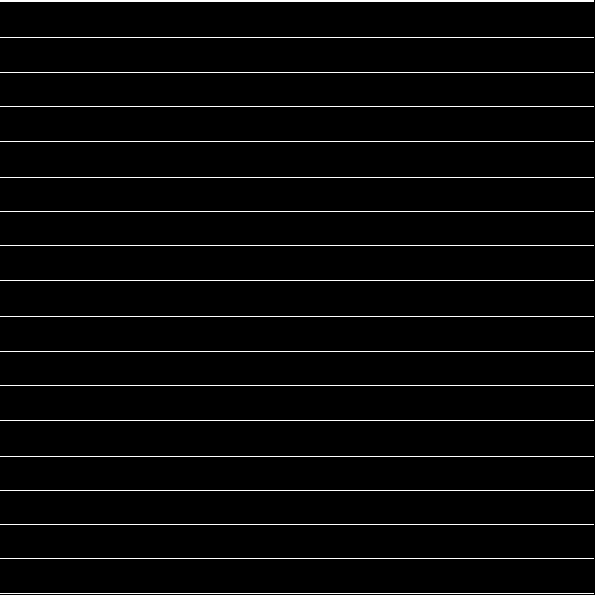
\includegraphics[width=\linewidth]{ressources/1step_09_horizontal_lines.png}
      \caption{}
    \endminipage\quad\quad\quad\quad
    \minipage{0.30\textwidth}
    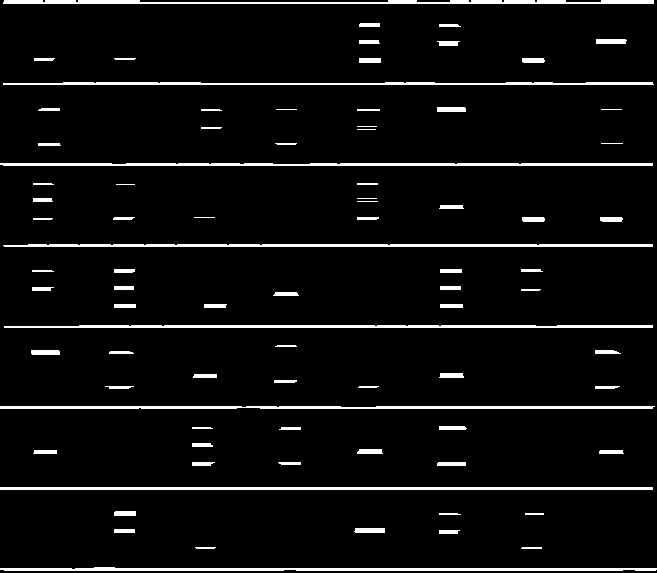
\includegraphics[width=\linewidth]{ressources/3step_09_horizontal_lines.png}
    \caption{}
  \endminipage
  \caption{Détection des lignes horizontales.}
\end{figure}


\begin{figure}[H]
  \centering
  \minipage{0.30\textwidth}
      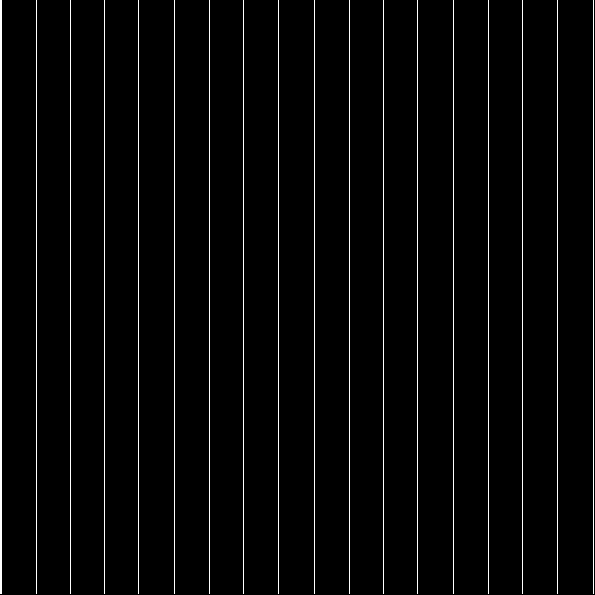
\includegraphics[width=\linewidth]{ressources/1step_09_vertical_lines.png}
      \caption{}
    \endminipage\quad\quad\quad\quad
    \minipage{0.30\textwidth}
    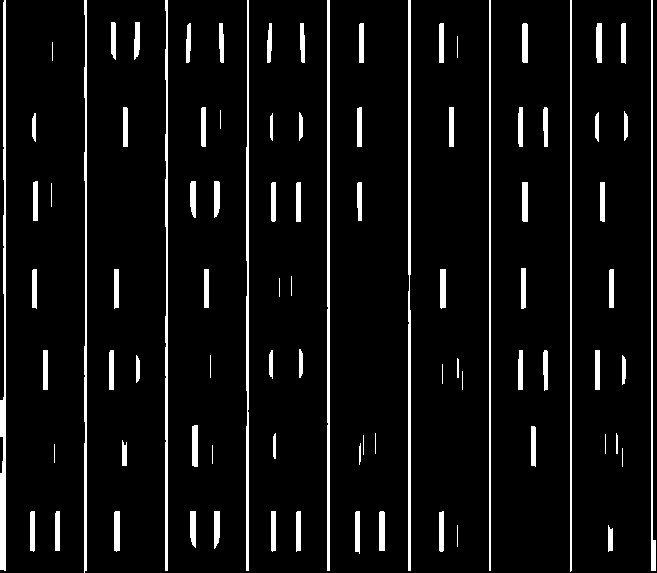
\includegraphics[width=\linewidth]{ressources/3step_09_vertical_lines.png}
    \caption{}
  \endminipage
  \caption{Détection des lignes verticales.}
\end{figure}
Cette méthode est utilisée lorsque l'image de la grille contient des lignes horizontales et verticales clairement visibles qui délimitent les cellules.

\paragraph{1. Détection des lignes}
Pour extraire les lignes, nous utilisons une opération spécialisée appelée \texttt{ouverture morphologique}. Celle-ci est particulièrement efficace pour supprimer les petits objets d'une image tout en préservant la forme et la taille des objets plus grands. L'opération se déroule en deux temps, en utilisant un noyau (ou "élément structurant") adapté à la forme que l'on souhaite conserver.

\begin{itemize}
    \item \textbf{Pour les lignes horizontales}, on utilise un élément structurant très large et fin (par exemple, de 40x1 pixels).
    \begin{enumerate}
        \item \textbf{Étape d'érosion :} L'image est d'abord érodée avec ce noyau horizontal. Rappelons que l'érosion amincit les formes. Comme le noyau est très large, tout objet blanc qui est plus fin que 40 pixels horizontalement (comme les lettres, le bruit, ou les lignes verticales) sera complètement "rongé" et disparaîtra. Seules les longues lignes horizontales survivront à cette étape, bien qu'elles soient amincies.
        \item \textbf{Étape de dilatation :} L'image résultante (ne contenant que des lignes horizontales amincies) est ensuite dilatée avec le même noyau. La dilatation épaissit les formes. Cette étape a pour effet de restaurer les lignes horizontales à leur épaisseur d'origine.
    \end{enumerate}
    Le résultat net de cette ouverture est une image ne contenant que les lignes horizontales de la grille.

    \item \textbf{Pour les lignes verticales}, le principe est identique, mais on utilise un élément structurant très haut et étroit (par exemple, 1x40 pixels).
    \begin{enumerate}
        \item \textbf{Étape d'érosion :} L'érosion avec ce noyau vertical supprime tous les objets qui ne sont pas de longues lignes verticales.
        \item \textbf{Étape de dilatation :} La dilatation qui suit restaure l'épaisseur des lignes verticales qui ont survécu.
    \end{enumerate}
\end{itemize}


\paragraph{2. Détermination des frontières}
Une fois les images des lignes obtenues, les frontières des cellules sont déterminées en analysant les projections de ces images. On scanne chaque ligne (pour les frontières horizontales) et chaque colonne (pour les frontières verticales) pour identifier les positions exactes des lignes détectées. Ces positions deviennent les délimitations des cellules.

\subsubsection{Cas 2 : Grille sans lignes internes (Détection par Lettres)}

\begin{figure}[H]
  \centering
  \minipage{0.30\textwidth}
      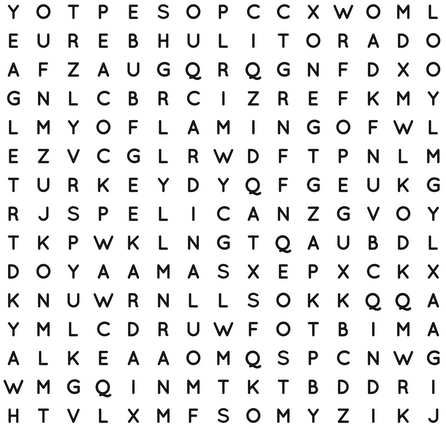
\includegraphics[width=\linewidth]{ressources/3step_08_text_region.png}
      \caption{}
    \endminipage\hfill
\end{figure}
Lorsque la grille ne contient pas de lignes internes, nous devons déduire sa structure en nous basant sur la disposition des lettres elles-mêmes.

\paragraph{1. Localisation de la région de texte}
D'abord, nous détectons tous les contours dans l'image de la grille et nous les filtrons pour ne garder que ceux qui ressemblent à des lettres (en se basant sur leur taille, leur forme, etc.). Ensuite, nous calculons la boîte englobante de l'ensemble de ces contours de lettres. Cette boîte définit la "région de texte", qui est une version plus précise de la grille, débarrassée des marges vides.


\paragraph{2. Inférence des dimensions de la grille}
Pour déduire le nombre de lignes et de colonnes à partir des positions des lettres, un algorithme de clustering est utilisé. L'idée est de regrouper les lettres qui sont alignées. L'algorithme traite les coordonnées Y et X des centres des lettres de manière indépendante. D'abord, il groupe les coordonnées Y qui sont très proches pour déterminer le nombre de lignes distinctes. Ensuite, il répète le processus sur les coordonnées X pour trouver le nombre de colonnes. Le nombre de groupes finaux pour chaque axe nous donne les dimensions de la grille.

\paragraph{3. Création d'une grille virtuelle}
Connaissant les dimensions de la région de texte et le nombre de lignes et de colonnes, nous pouvons générer une grille virtuelle en divisant simplement la région en cellules de taille égale.

\subsubsection{Résultat : La grille segmentée}

Quelle que soit la méthode utilisée, le résultat final est une série de coordonnées qui définissent les frontières de chaque cellule de la grille. Cela nous permet de "découper" chaque lettre individuellement pour la reconnaissance de caractères.

\begin{figure}[H]
    \stepimage[0.30\textwidth]{1step_10_reconstructed_grid.png}{}
    \stepimage[0.33\textwidth]{2step_10_reconstructed_grid.png}{}
    \stepimage[0.26\textwidth]{3step_10_reconstructed_grid.png}{}
    \caption{Grille segmentée avec les frontières des cellules détectées.}
\end{figure}

\section{Extraction de la Liste de Mots}
L'étape finale consiste à extraire la liste des mots à rechercher à partir d'une région de l'image. Ce processus est une chaîne de traitement d'image à part entière, conçue pour isoler des lignes de texte.

\subsection{Pré-traitement et Binarisation}
\paragraph{1. Préparation de l'image}
Comme pour la grille, l'image est d'abord convertie en niveaux de gris et un léger flou gaussien est appliqué pour réduire le bruit et lisser les caractères.

\paragraph{2. Binarisation par Combinaison}
Le texte peut être difficile à segmenter à cause des variations d'éclairage, des ombres ou de la qualité de l'impression. Pour surmonter cela, au lieu d'une seule méthode de seuillage, nous en combinons trois pour maximiser nos chances de capturer tout le texte :

  \begin{itemize}
    \item \textbf{Méthode d'Otsu :} C'est un algorithme de seuillage global automatique. Plutôt que d'utiliser une valeur fixe, l'algorithme d'Otsu analyse l'histogramme des intensités de tous les pixels de l'image. Il parcourt tous les seuils possibles (de 0 à 255) et, pour chaque seuil, il calcule la variance des pixels des deux classes qu'il créerait (premier-plan et arrière-plan). Le seuil optimal est celui qui \textbf{minimise la variance intra-classe} (ou, de manière équivalente, maximise la variance inter-classe). Il est très efficace pour les images bimodales (comme du texte noir sur un fond clair).
    \begin{figure}[H]
      \centering
      \minipage{0.29\textwidth}
          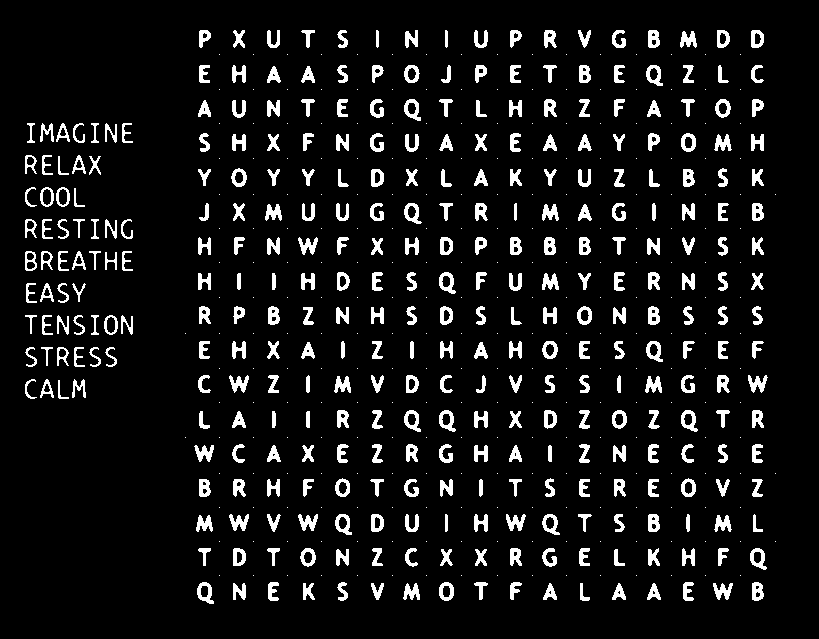
\includegraphics[width=\linewidth]{ressources/1level_1_image_1_03_otsu_threshold.png}
          \caption{}
        \endminipage\quad\quad\quad\quad
        \minipage{0.25\textwidth}
        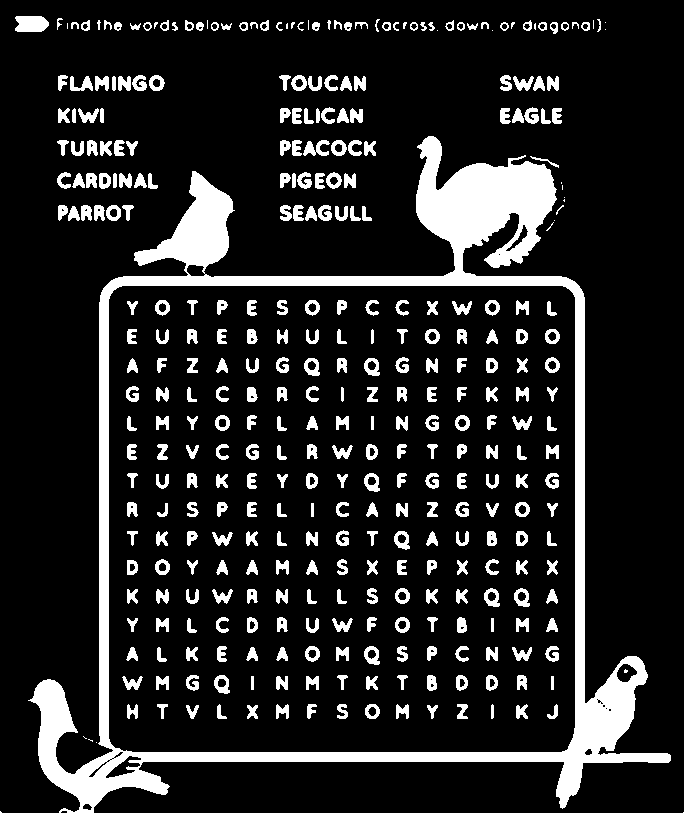
\includegraphics[width=\linewidth]{ressources/3level_3_image_2_03_otsu_threshold.png}
        \caption{}
      \endminipage
      \caption{Seuillage par Otsu.}
    \end{figure}

    \item \textbf{Seuillage Adaptatif Gaussien :} Comme vu précédemment, cette méthode calcule un seuil local pour chaque pixel en se basant sur une moyenne pondérée gaussienne de son voisinage. Elle excelle dans la gestion des gradients d'éclairage.
    \begin{figure}[H]
      \centering
      \minipage{0.29\textwidth}
          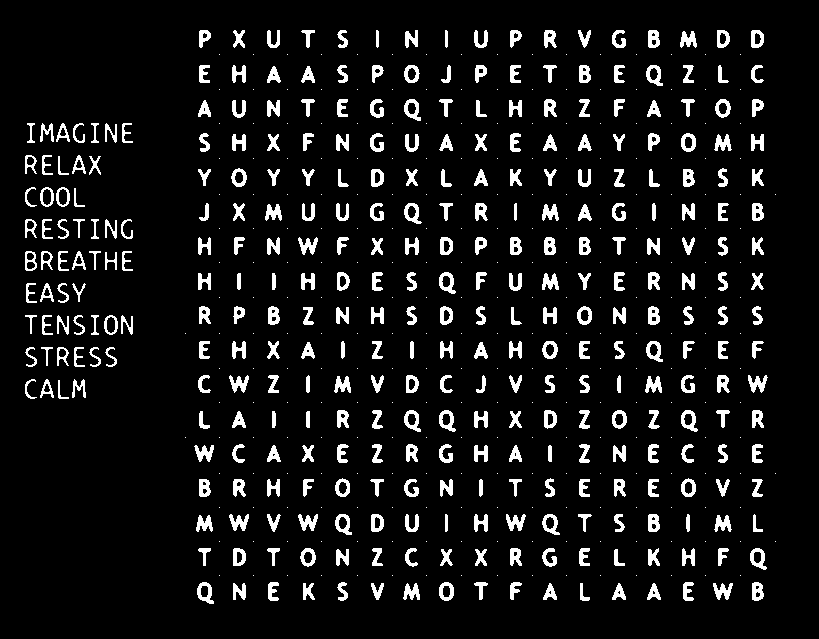
\includegraphics[width=\linewidth]{ressources/1level_1_image_1_04_adaptive_threshold.png}
          \caption{}
        \endminipage\quad\quad\quad\quad
        \minipage{0.25\textwidth}
        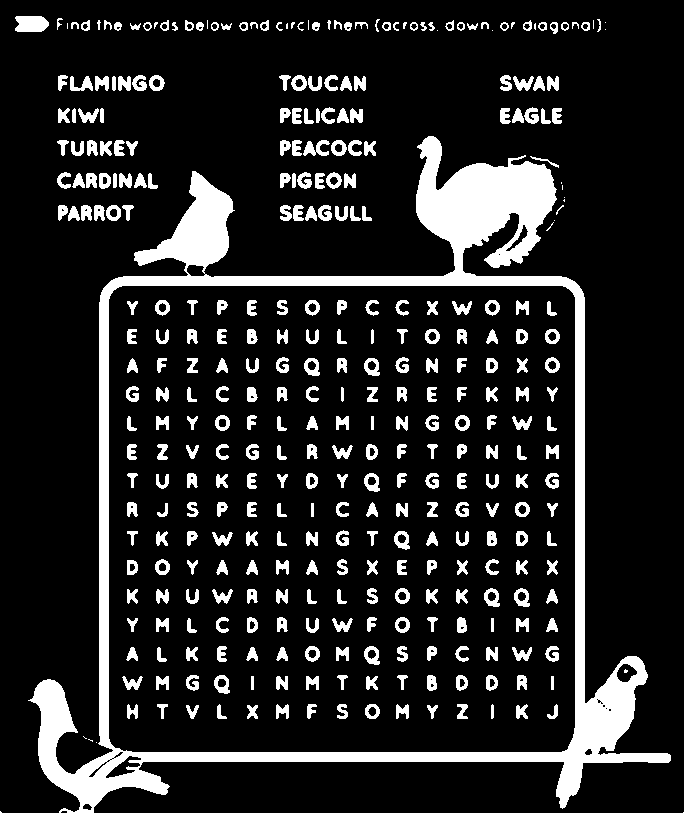
\includegraphics[width=\linewidth]{ressources/3level_3_image_2_04_adaptive_threshold.png}
        \caption{}
      \endminipage
      \caption{Seuillage adaptatif.}
    \end{figure}
    \item \textbf{Seuillage par la Moyenne :} Une version plus simple du seuillage global, où le seuil est calculé comme un pourcentage (par exemple, 80\%) de l'intensité moyenne de tous les pixels de l'image.
    \begin{figure}[H]
      \centering
      \minipage{0.29\textwidth}
          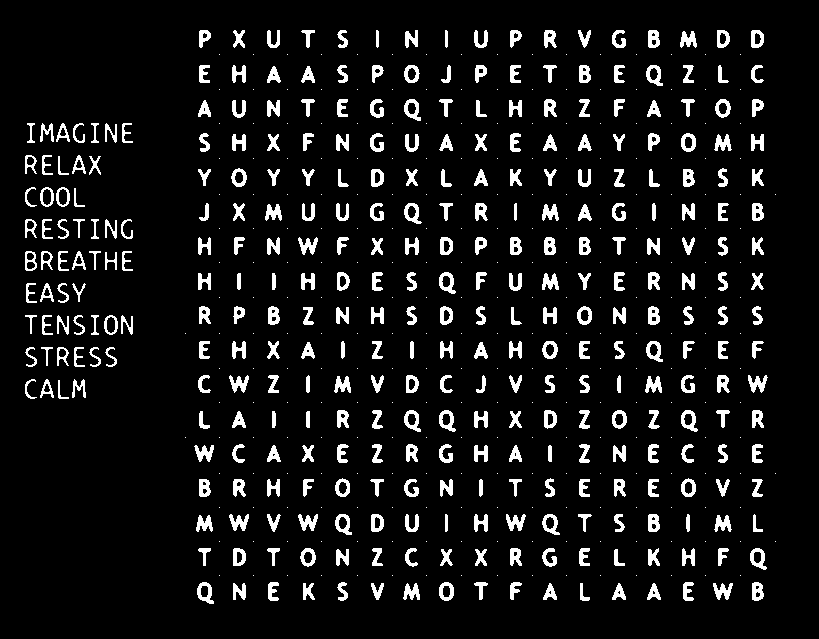
\includegraphics[width=\linewidth]{ressources/1level_1_image_1_05_mean_threshold.png}
          \caption{}
        \endminipage\quad\quad\quad\quad
        \minipage{0.25\textwidth}
        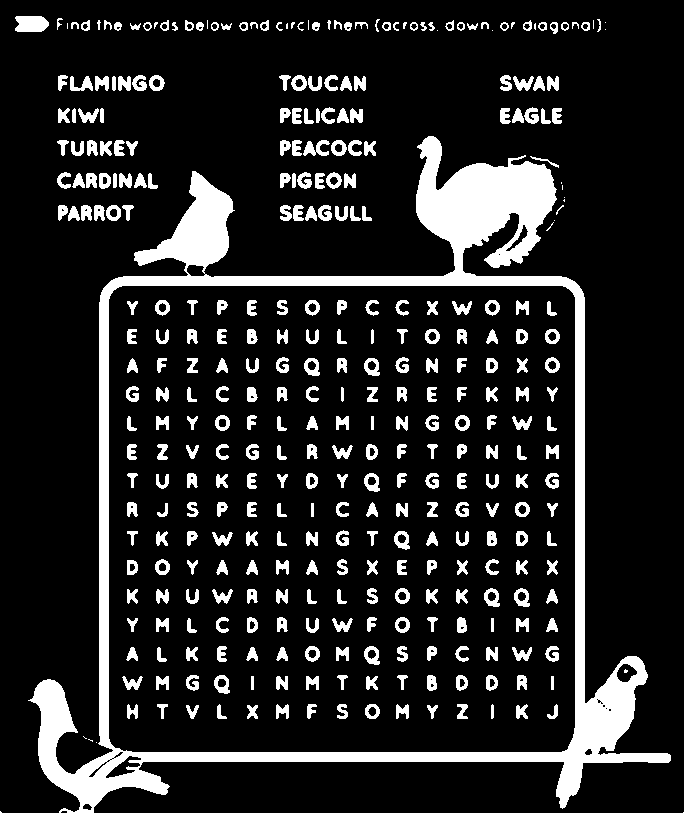
\includegraphics[width=\linewidth]{ressources/3level_3_image_2_05_mean_threshold.png}
        \caption{}
      \endminipage
      \caption{Seuillage adaptatif.}
    \end{figure}
\end{itemize}

\paragraph{3. Fusion des Résultats}
Les trois images binaires résultantes sont ensuite fusionnées en une seule image en utilisant une opération \texttt{OU} logique pixel à pixel. Un pixel est considéré comme faisant partie du texte dans l'image finale s'il a été classé comme tel par \textit{au moins une} des trois méthodes..
\begin{figure}[H]
  \centering
  \minipage{0.29\textwidth}
      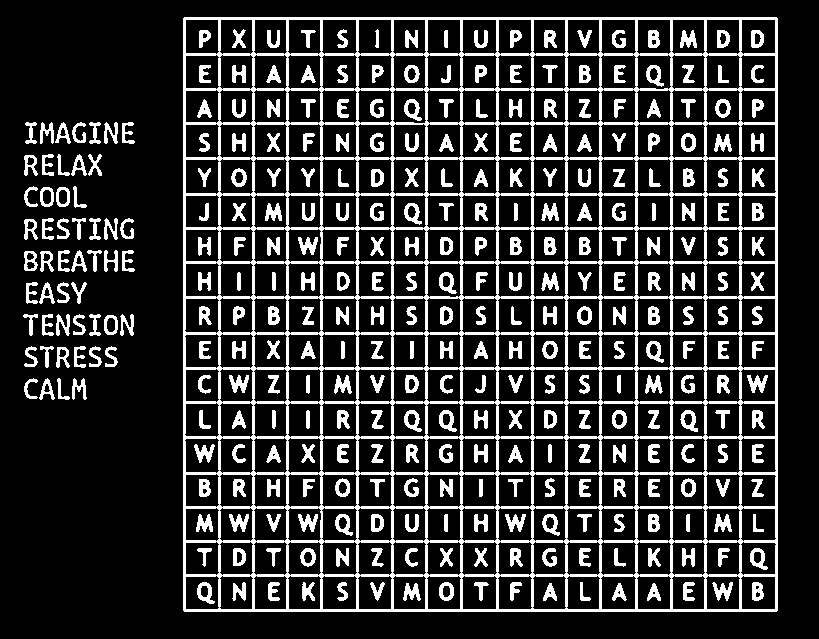
\includegraphics[width=\linewidth]{ressources/1level_1_image_1_06_combined_threshold.png}
      \caption{}
    \endminipage\quad\quad\quad\quad
    \minipage{0.25\textwidth}
    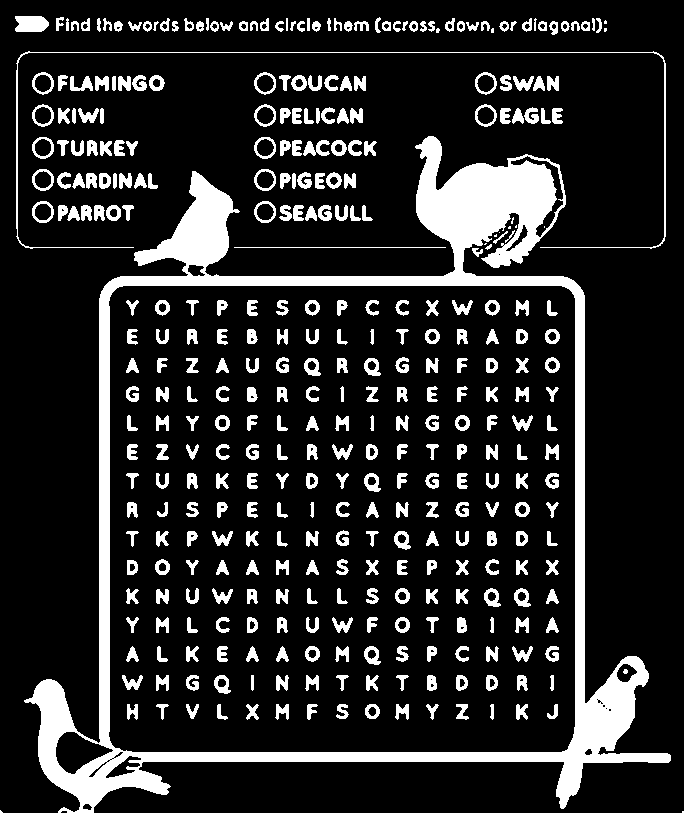
\includegraphics[width=\linewidth]{ressources/3level_3_image_2_06_combined_threshold.png}
    \caption{}
  \endminipage
  \caption{Fusion des résultats.}
\end{figure}
\subsection{Analyse et Groupement des Mots}
Une fois l'image binarisée, des opérations morphologiques sont appliquées pour transformer les lettres individuelles en des "blobs" solides correspondant à des mots entiers. Une séquence de \texttt{fermeture}, de \texttt{dilatation} et d'\texttt{érosion} permet de combler les trous dans les lettres et de connecter les caractères adjacents.

\begin{figure}[H]
  \centering
  \minipage{0.29\textwidth}
      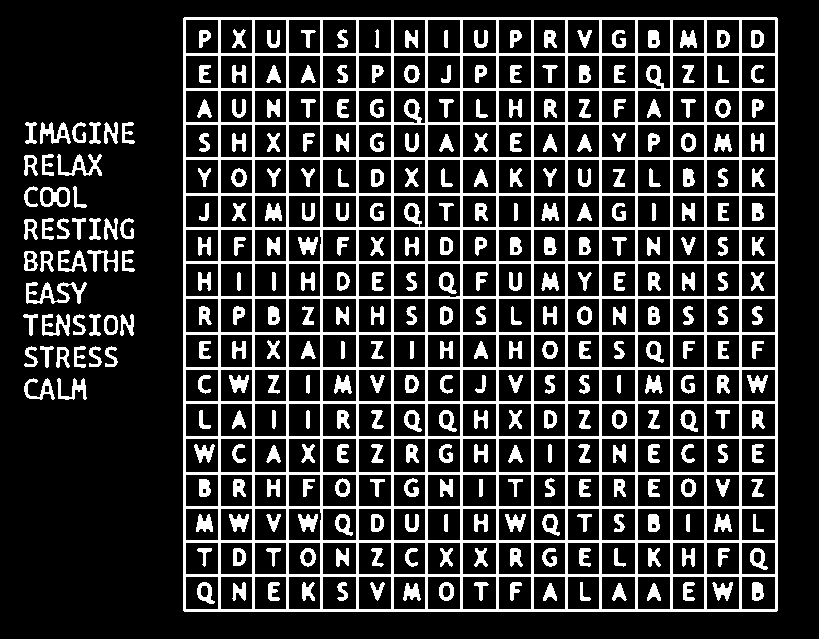
\includegraphics[width=\linewidth]{ressources/1level_1_image_1_07_morphology_closed.png}
      \caption{}
    \endminipage\quad\quad\quad\quad
    \minipage{0.25\textwidth}
    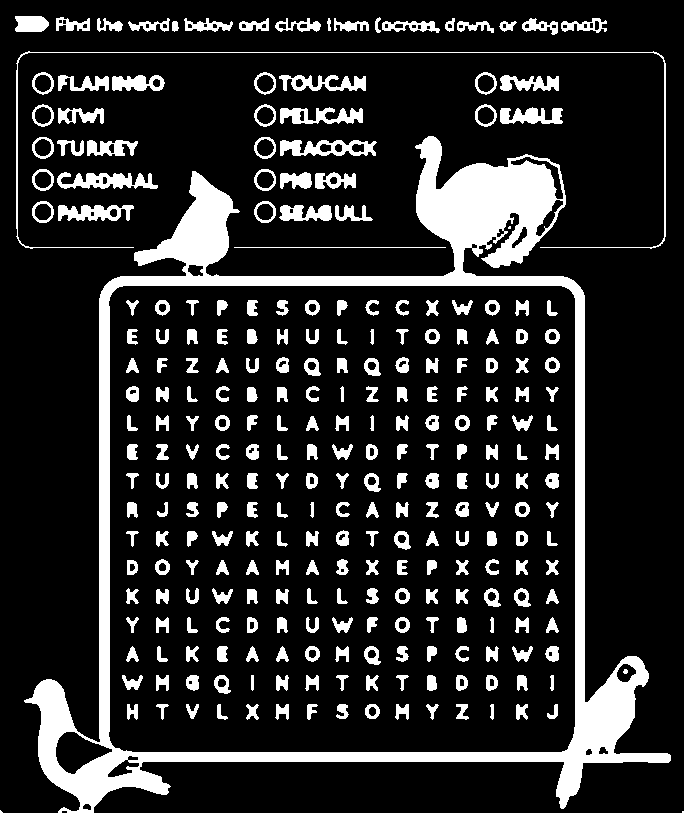
\includegraphics[width=\linewidth]{ressources/3level_3_image_2_07_morphology_closed.png}
    \caption{}
  \endminipage
  \caption{Fermeture morphologique.}
\end{figure}
\begin{figure}[H]
  \centering
  \minipage{0.29\textwidth}
      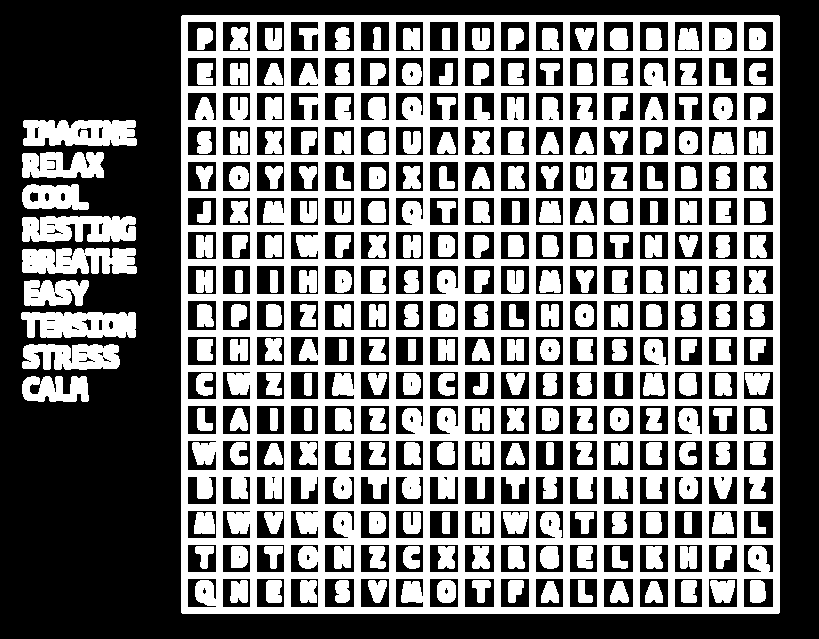
\includegraphics[width=\linewidth]{ressources/1level_1_image_1_08_dilated.png}
      \caption{}
    \endminipage\quad\quad\quad\quad
    \minipage{0.25\textwidth}
    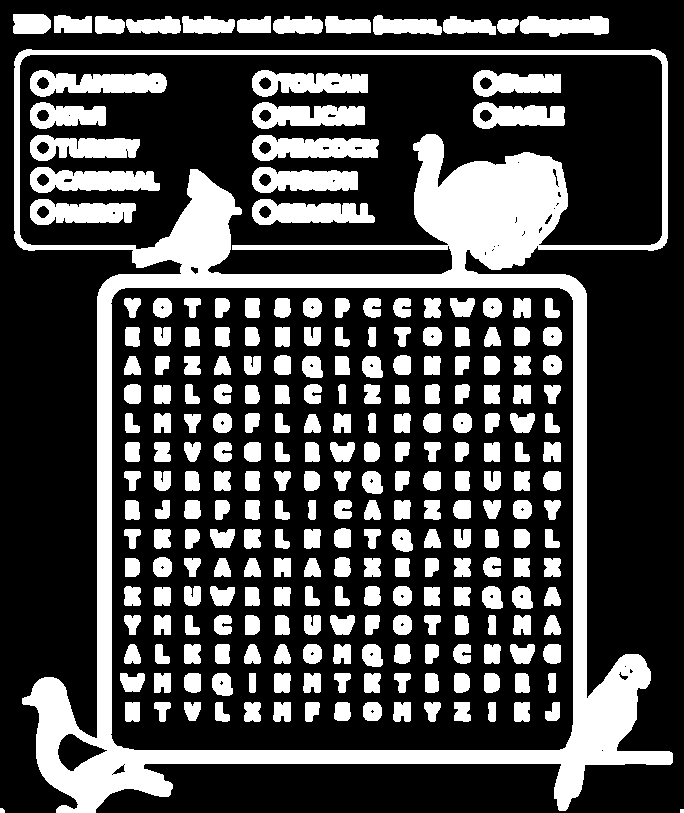
\includegraphics[width=\linewidth]{ressources/3level_3_image_2_08_dilated.png}
    \caption{}
  \endminipage
  \caption{Dilatation.}
\end{figure}
\begin{figure}[H]
  \centering
  \minipage{0.29\textwidth}
      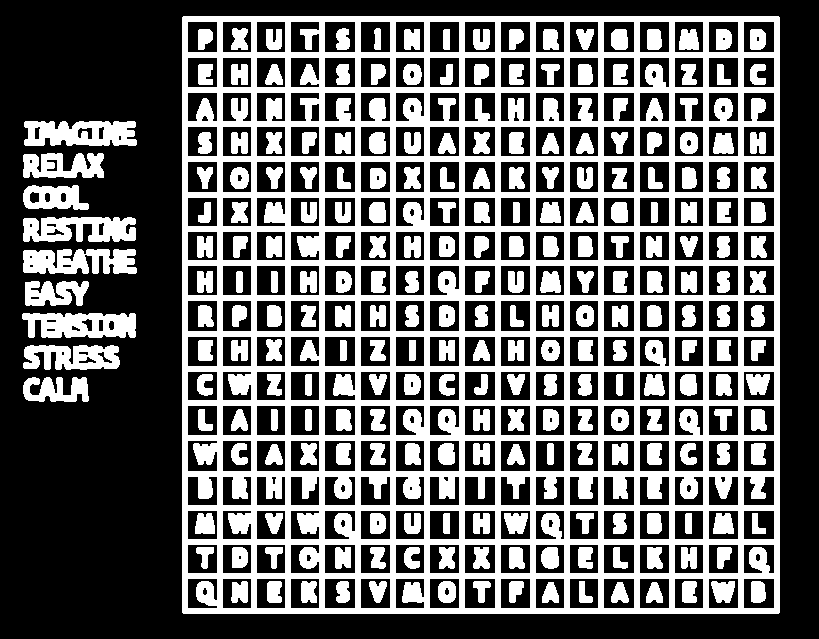
\includegraphics[width=\linewidth]{ressources/1level_1_image_1_09_eroded.png}
      \caption{}
    \endminipage\quad\quad\quad\quad
    \minipage{0.25\textwidth}
    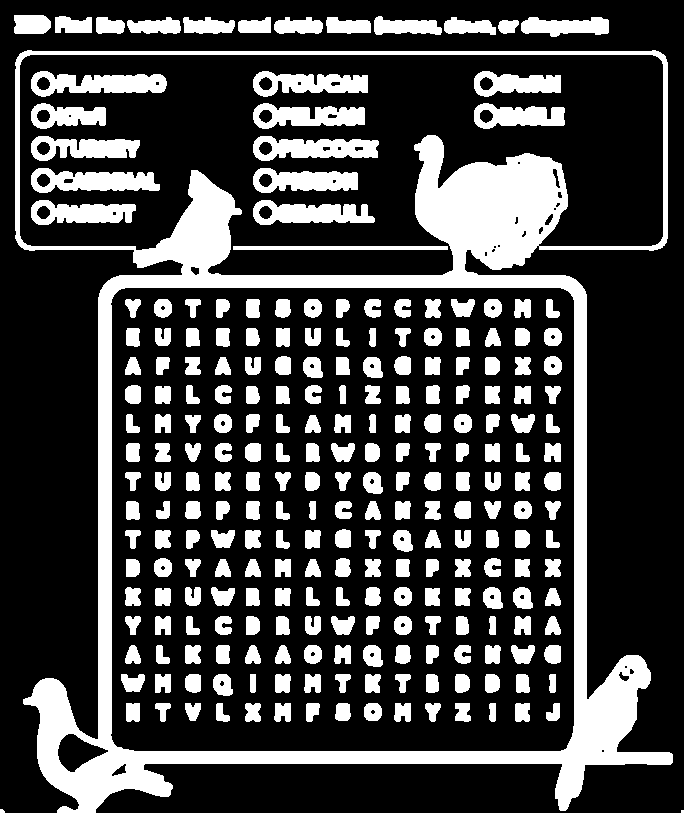
\includegraphics[width=\linewidth]{ressources/3level_3_image_2_09_eroded.png}
    \caption{}
  \endminipage
  \caption{Érosion.}
\end{figure}
\paragraph{1. Détection et Filtrage :} Comme précédemment, les contours de tous les "blobs" sont détectés, et ceux qui ne correspondent pas à des critères géométriques de mots (taille, ratio, etc.) sont éliminés.

\paragraph{2. Algorithme de Fusion Horizontale :} Pour regrouper les fragments de mots, un algorithme de fusion est appliqué :
\begin{enumerate}
    \item Les boîtes englobantes de tous les contours restants sont triées par leur coordonnée X.
    \item L'algorithme parcourt la liste triée, en maintenant une "boîte courante". Pour chaque boîte suivante, il calcule l'écart horizontal et le chevauchement vertical avec la boîte courante.
    \item Si l'écart est faible ET que le chevauchement est important (ce qui signifie que les deux boîtes sont proches et sur la même ligne), elles sont fusionnées en une seule boîte plus grande qui devient la nouvelle "boîte courante".
    \item Sinon, la "boîte courante" est finalisée et ajoutée à la liste des mots, et la boîte suivante devient la nouvelle "boîte courante".
    \item Ce processus garantit que seules les boîtes adjacentes et bien alignées sont fusionnées pour former des mots complets.
\end{enumerate}

\paragraph{3. Regroupement en Lignes et Sélection du Bloc Principal}
Enfin, les boîtes des mots fusionnés sont regroupées pour identifier la liste de mots principale.
\begin{enumerate}
    \item \textbf{Regroupement en lignes :} D'abord, un algorithme de clustering (similaire à celui vu pour la grille) est utilisé pour regrouper les mots en lignes, en se basant sur l'alignement vertical de leurs centres.

    \item \textbf{Analyse de l'espacement vertical :} L'algorithme calcule ensuite l'écart vertical moyen entre chaque ligne consécutive. Il identifie l'espacement le plus fréquent, qui correspond à l'interligne standard du bloc de texte principal.

    \item \textbf{Regroupement en blocs :} En se basant sur cet interligne standard, l'algorithme regroupe les lignes consécutives en blocs. Une rupture (un écart vertical beaucoup plus grand que la norme) signale la fin d'un bloc et le début d'un autre.

    \item \textbf{Sélection finale :} L'algorithme part du principe que la liste de mots à rechercher est le bloc de texte le plus dense. Il sélectionne donc le bloc qui contient le plus grand nombre de mots. Le résultat est un ensemble final de boîtes englobantes, chacune correspondant à un mot à trouver.
\end{enumerate}
\begin{figure}[H]
  \centering
  \minipage{0.29\textwidth}
      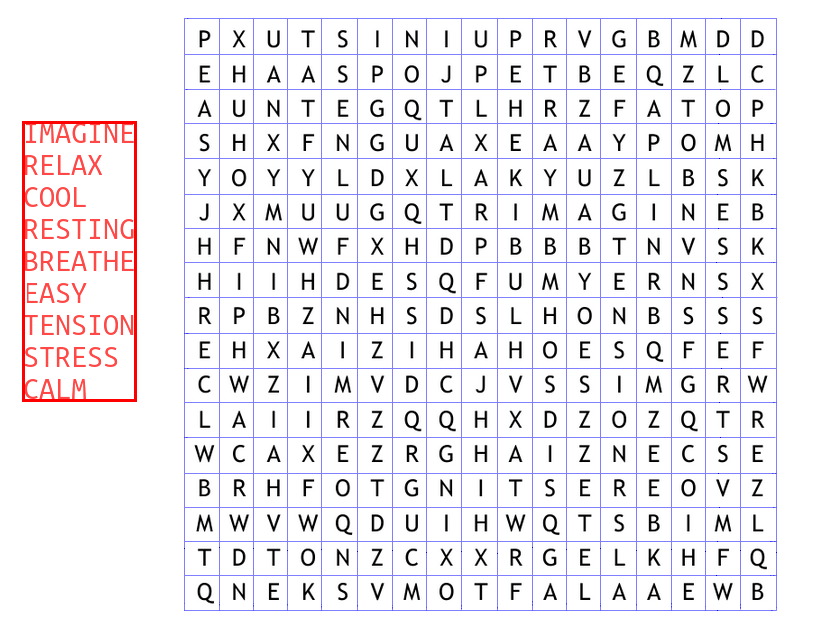
\includegraphics[width=\linewidth]{ressources/words_with_squares_level_1_image_1.png}
      \caption{}
    \endminipage\quad\quad\quad\quad
    \minipage{0.25\textwidth}
    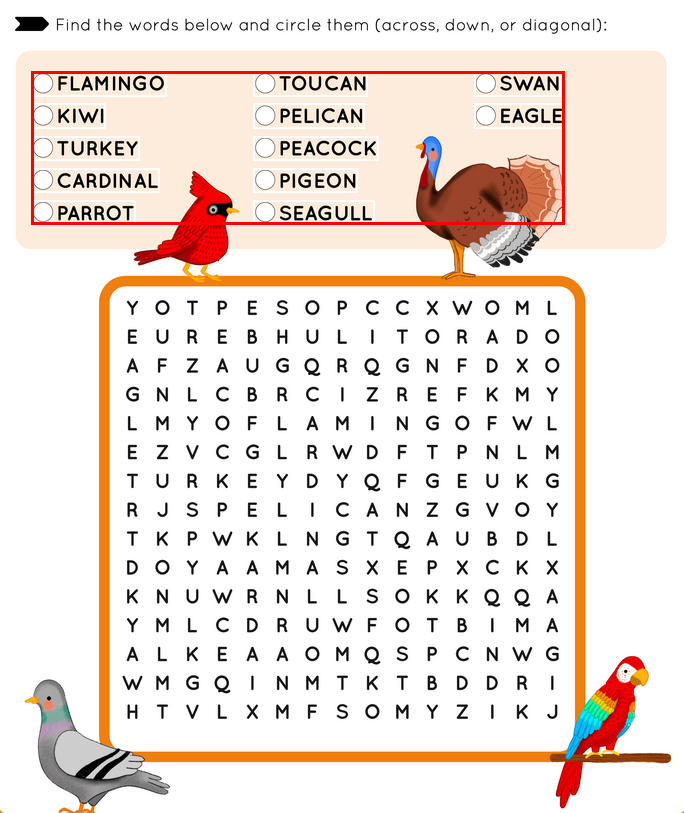
\includegraphics[width=\linewidth]{ressources/words_with_squares_level_3_image_2.png}
    \caption{}
  \endminipage
  \caption{Détection des mots.}
\end{figure}

\end{document}
